% !TeX program = xelatex
\documentclass[UTF8,a4paper,9pt,twocolumn,fontset=none]{ctexart}

\usepackage{iftex}
\ifXeTeX\else
  \PackageError{market-report}{This document must be compiled with XeLaTeX}
  {In Overleaf, open Menu -> Settings -> Compiler and select XeLaTeX.}
\fi
\setCJKmainfont{FandolSong-Regular}
\setCJKsansfont{FandolHei-Regular}
\setCJKmonofont{FandolFang-Regular}

\usepackage[left=1.35cm,right=1.35cm,top=1.35cm,bottom=1.45cm,columnsep=0.62cm]{geometry}
\usepackage{amsmath,amssymb,booktabs,tabularx,array,multirow}
\usepackage{graphicx,subcaption,float,enumitem,hyperref,xcolor,microtype}
\usepackage{tikz}
\usetikzlibrary{arrows.meta,positioning,shapes.geometric}

\hypersetup{
  colorlinks=true,
  linkcolor=black,
  citecolor=blue!55!black,
  urlcolor=blue!55!black
}
\setlength{\parindent}{2em}
\setlength{\parskip}{0pt}
\setlength{\columnsep}{0.62cm}
\setlength{\floatsep}{5pt plus 1pt minus 1pt}
\setlength{\textfloatsep}{6pt plus 1pt minus 1pt}
\setlength{\intextsep}{5pt plus 1pt minus 1pt}
\setlength{\abovecaptionskip}{3pt}
\setlength{\belowcaptionskip}{0pt}
\setlist{nosep,leftmargin=1.45em}
\renewcommand{\baselinestretch}{0.97}
\newcolumntype{Y}{>{\raggedright\arraybackslash}X}
\pagestyle{plain}

\ctexset{
  section={format=\large\bfseries,beforeskip=5pt,afterskip=2pt},
  subsection={format=\normalsize\bfseries,beforeskip=3pt,afterskip=1pt}
}
\captionsetup{font=small,labelfont=bf}

\title{\vspace{-1.2cm}\textbf{基于金融新闻情绪与股票价格数据的市场趋势预测研究}}
\author{黄文轩\quad 王子轩\quad 林瀚羽\quad 彭琰轲\\
\small 深圳大学金融科技专业}
\date{}

\begin{document}

\maketitle
\vspace{-1.7em}
\begin{abstract}
\small
金融市场会对新闻中的新增信息与投资者预期作出反应，但新闻情绪是否具有稳定的
样本外预测价值仍存在争议。本文基于Combined News and DJIA公开数据，将2008年
8月至2016年7月每日25条新闻标题与道琼斯工业平均指数（DJIA）行情匹配。为避免
同日新闻与收盘价之间的时点歧义，使用$t$日新闻情绪和截至$t$日可观测的量价指标，
预测$t+1$日指数方向。本文以VADER提取情绪，构造情绪均值、分歧、正负占比和
滞后变化等变量，比较Logistic回归、随机森林与XGBoost在“仅量价”和
“量价+新闻”两组特征下的表现。2014--2016年walk-forward实验表明，XGBoost加入
新闻后平均ROC-AUC由0.472提高至0.504，但AUC增量的95\% bootstrap置信区间为
$[-0.006,0.073]$，未达到统计显著。新闻策略扣除10个基点仓位调整成本后的年化
收益为$-13.1\%$，夏普比率为$-1.51$。年度稳定性、相关性、概率校准和阈值敏感性
分析进一步显示，新闻情绪至多提供微弱且时变的非线性信息，尚不足以支持稳定交易。

\noindent\textbf{关键词：}金融新闻；情绪分析；VADER；股票趋势预测；XGBoost；
walk-forward验证
\end{abstract}
\vspace{0.4em}

\section{引言}

股票市场具有高度信息驱动特征。传统预测通常使用收益率、成交量、移动平均线和
波动率等结构化变量，但公司事件、宏观政策、地缘冲突和媒体叙事也会改变投资者预期。
Tetlock发现媒体悲观语调与市场收益及交易量存在关系\cite{tetlock}；
Loughran和McDonald进一步表明，通用情感词典会误判大量金融术语，领域语境不可
忽略\cite{lm}。

近年来，文本预测研究从词典计数发展到事件表示、神经网络和预训练语言模型。
Ding等将新闻事件转换为稠密表示并用于指数预测\cite{ding2015}；StockNet联合
社交文本与历史价格建模\cite{stocknet}；FinBERT通过金融语料适配提升金融情绪
分类能力\cite{finbert}；FNSPID和CausalStock则进一步面向大规模、多股票和关系
建模\cite{fnspid,causalstock}。这些工作说明新闻与价格融合具有研究价值，但也
意味着预测效果高度依赖数据规模、时间戳质量、文本与公司的匹配粒度。

公开教学数据常只有每日新闻标题而没有精确发布时间。若直接用当天全部标题预测
当天收盘标签，模型可能读取收盘后新闻；若随机拆分时间序列，未来市场状态会进入
训练集。为降低这两类偏差，本文将任务重新定义为严格的下一交易日预测，并采用
递增窗口和隔离期。

本文贡献包括：（1）构造新闻情绪与量价特征的可复现实验管线；（2）以特征消融
直接检验新闻的增量价值；（3）同时报告统计显著性、年度稳定性、概率校准和经济
回测；（4）如实分析接近随机和回测失败的结果，避免只展示表现最好的窗口。

\begin{figure*}[t]
\centering
\begin{tikzpicture}[
  node distance=0.28cm,
  box/.style={draw,rounded corners,align=center,minimum height=1.0cm,
              text width=2.30cm,fill=blue!5,font=\small},
  arrow/.style={-{Latex[length=2mm]},thick}
]
\node[box] (news) {每日Top 25新闻\\文本清洗与VADER};
\node[box,right=of news] (sent) {日度情绪特征\\均值、分歧、正负占比};
\node[box,right=of sent] (price) {DJIA行情特征\\收益、波动、量价指标};
\node[box,right=of price] (panel) {时间对齐面板\\$t$日特征预测$t+1$};
\node[box,right=of panel] (model) {LR / RF / XGBoost\\P与P+N消融};
\node[box,right=of model] (eval) {walk-forward\\统计检验与回测};
\draw[arrow] (news)--(sent);
\draw[arrow] (sent)--(price);
\draw[arrow] (price)--(panel);
\draw[arrow] (panel)--(model);
\draw[arrow] (model)--(eval);
\end{tikzpicture}
\caption{本文的数据处理、建模与验证流程}
\label{fig:workflow}
\end{figure*}

\section{文献综述}

\subsection{词典、情绪分类与金融语义}

早期金融文本研究多使用正负词频。Tetlock以媒体悲观词比例刻画市场情绪
\cite{tetlock}。Loughran--McDonald词典针对公司报告构建金融类别词汇，揭示
“liability”等词在一般语境与金融语境中的极性差异\cite{lm}。Financial
PhraseBank由金融专业人员标注句子情绪，是金融情绪分类常用基准\cite{phrasebank}。

VADER综合词典、否定、程度副词、大小写和标点规则，输出$[-1,1]$的compound
分数\cite{vader}。其优点是透明、无需训练且可完整复现，缺点是缺少金融领域
适配。FinBERT通过在金融语料上继续预训练并微调情绪分类，能更好处理上下文和
金融术语\cite{finbert}。本文选择VADER作为低成本基线，并将领域模型作为后续扩展。

\subsection{新闻驱动的市场预测}

Ding等使用事件抽取和深度卷积网络预测S\&P 500方向，强调事件结构比词袋更能表达
“谁对谁做了什么”\cite{ding2015}。StockNet将推文、用户信息与价格序列联合输入
变分循环模型，说明文本信号与价格动态可能存在时变交互\cite{stocknet}。
Akita等将新闻段落向量与股票价格结合，发现融合模型可能优于单一模态，但结果依赖
样本和市场\cite{akita}.

更近期研究转向大规模和关系建模。FNSPID整合千万级新闻与数千只股票价格，为
时间序列新闻研究提供更大数据基础\cite{fnspid}。CausalStock尝试从新闻和股票
关系中学习因果结构\cite{causalstock}。与这些数据相比，本文数据只有约2000个
交易日、且新闻是全球热点而非公司级事件，因此预期效果应更保守。

\subsection{研究假设}

\textbf{H1：}P+N模型的样本外AUC高于同算法P模型。\\
\textbf{H2：}新闻增量在不同测试年份保持同方向。\\
\textbf{H3：}若概率信号有效，扣除成本后应优于持有现金，并具有合理校准。

\section{数据与变量}

\subsection{数据来源与样本}

数据来自Kaggle的Daily News for Stock Market Prediction及公开镜像
\cite{dataset}。新闻表含\texttt{Date}和\texttt{Top1--Top25}；行情表含
DJIA开盘价、最高价、最低价、收盘价、成交量和复权收盘价。原始新闻表有1989日。
合并行情、构造20日滚动变量并删除末日无标签记录后，最终样本为1968日、
49193条有效标题，覆盖2008年9月8日至2016年6月30日。

\begin{table}[t]
\centering
\caption{样本描述统计}
\small
\begin{tabular}{lr}
\toprule
指标 & 数值\\
\midrule
交易日样本 & 1,968\\
有效新闻标题 & 49,193\\
平均每日标题数 & 25.00\\
下一日上涨比例 & 53.51\%\\
上涨日前情绪均值 & $-0.2150$\\
下跌日前情绪均值 & $-0.2168$\\
测试期样本数 & 575\\
\bottomrule
\end{tabular}
\label{tab:sample}
\end{table}

\subsection{新闻清洗与情绪特征}

清除Python字节串前缀、异常引号、HTML实体和多余空白。对第$t$日第$j$条标题
计算VADER分数$s_{j,t}$，日均情绪定义为：
\begin{equation}
\bar{s}_t=\frac{1}{N_t}\sum_{j=1}^{N_t}s_{j,t}.
\end{equation}
进一步构造情绪标准差、最小值、最大值、正向占比、负向占比、中性占比、滞后情绪
与情绪变化。VADER阈值采用官方常见规则：$s\geq0.05$为正向，
$s\leq-0.05$为负向。

\begin{figure}[t]
\centering
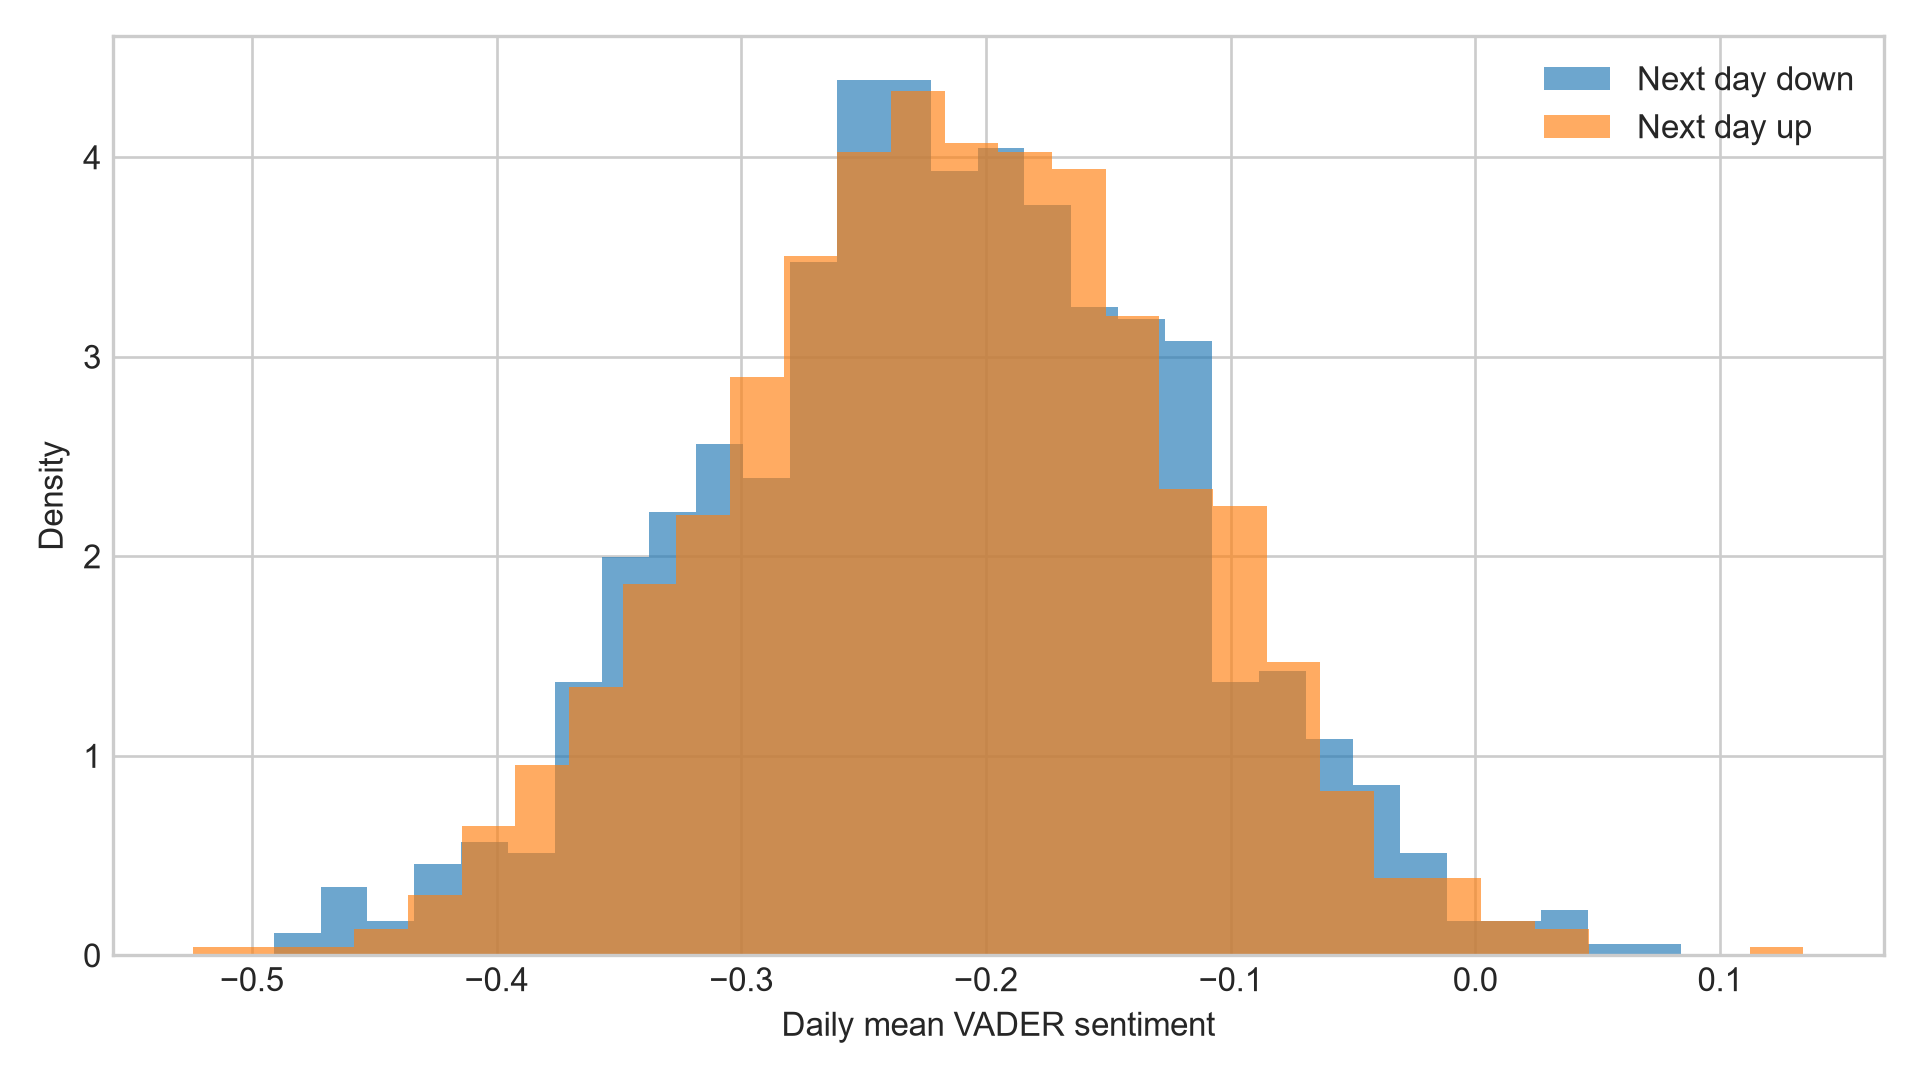
\includegraphics[width=\columnwidth]{figures/sentiment_distribution.png}
\caption{下一日上涨与下跌样本的日均新闻情绪分布}
\label{fig:sentdist}
\end{figure}

图\ref{fig:sentdist}显示两组分布高度重合。上涨日前与下跌日前平均情绪仅相差
0.0018，说明简单情绪均值难以形成线性可分信号。

\subsection{量价特征与标签}

以复权收盘价$P_t$计算$k$日收益率：
\begin{equation}
r_t^{(k)}=P_t/P_{t-k}-1.
\end{equation}
价格特征包括1/5/10/20日收益、5/20日均线差、5日和20日实现波动率、成交量变化、
日内振幅与5日动量方向。预测标签为：
\begin{equation}
y_{t+1}=\mathbb{I}(P_{t+1}/P_t-1>0).
\end{equation}
原数据同日标签不用于主实验。图\ref{fig:corr}中，日均情绪与下一日收益的相关系数
约为0.00，负面新闻占比约为$-0.04$；历史1日和5日收益与下一日收益均约为$-0.10$。

\begin{figure}[t]
\centering
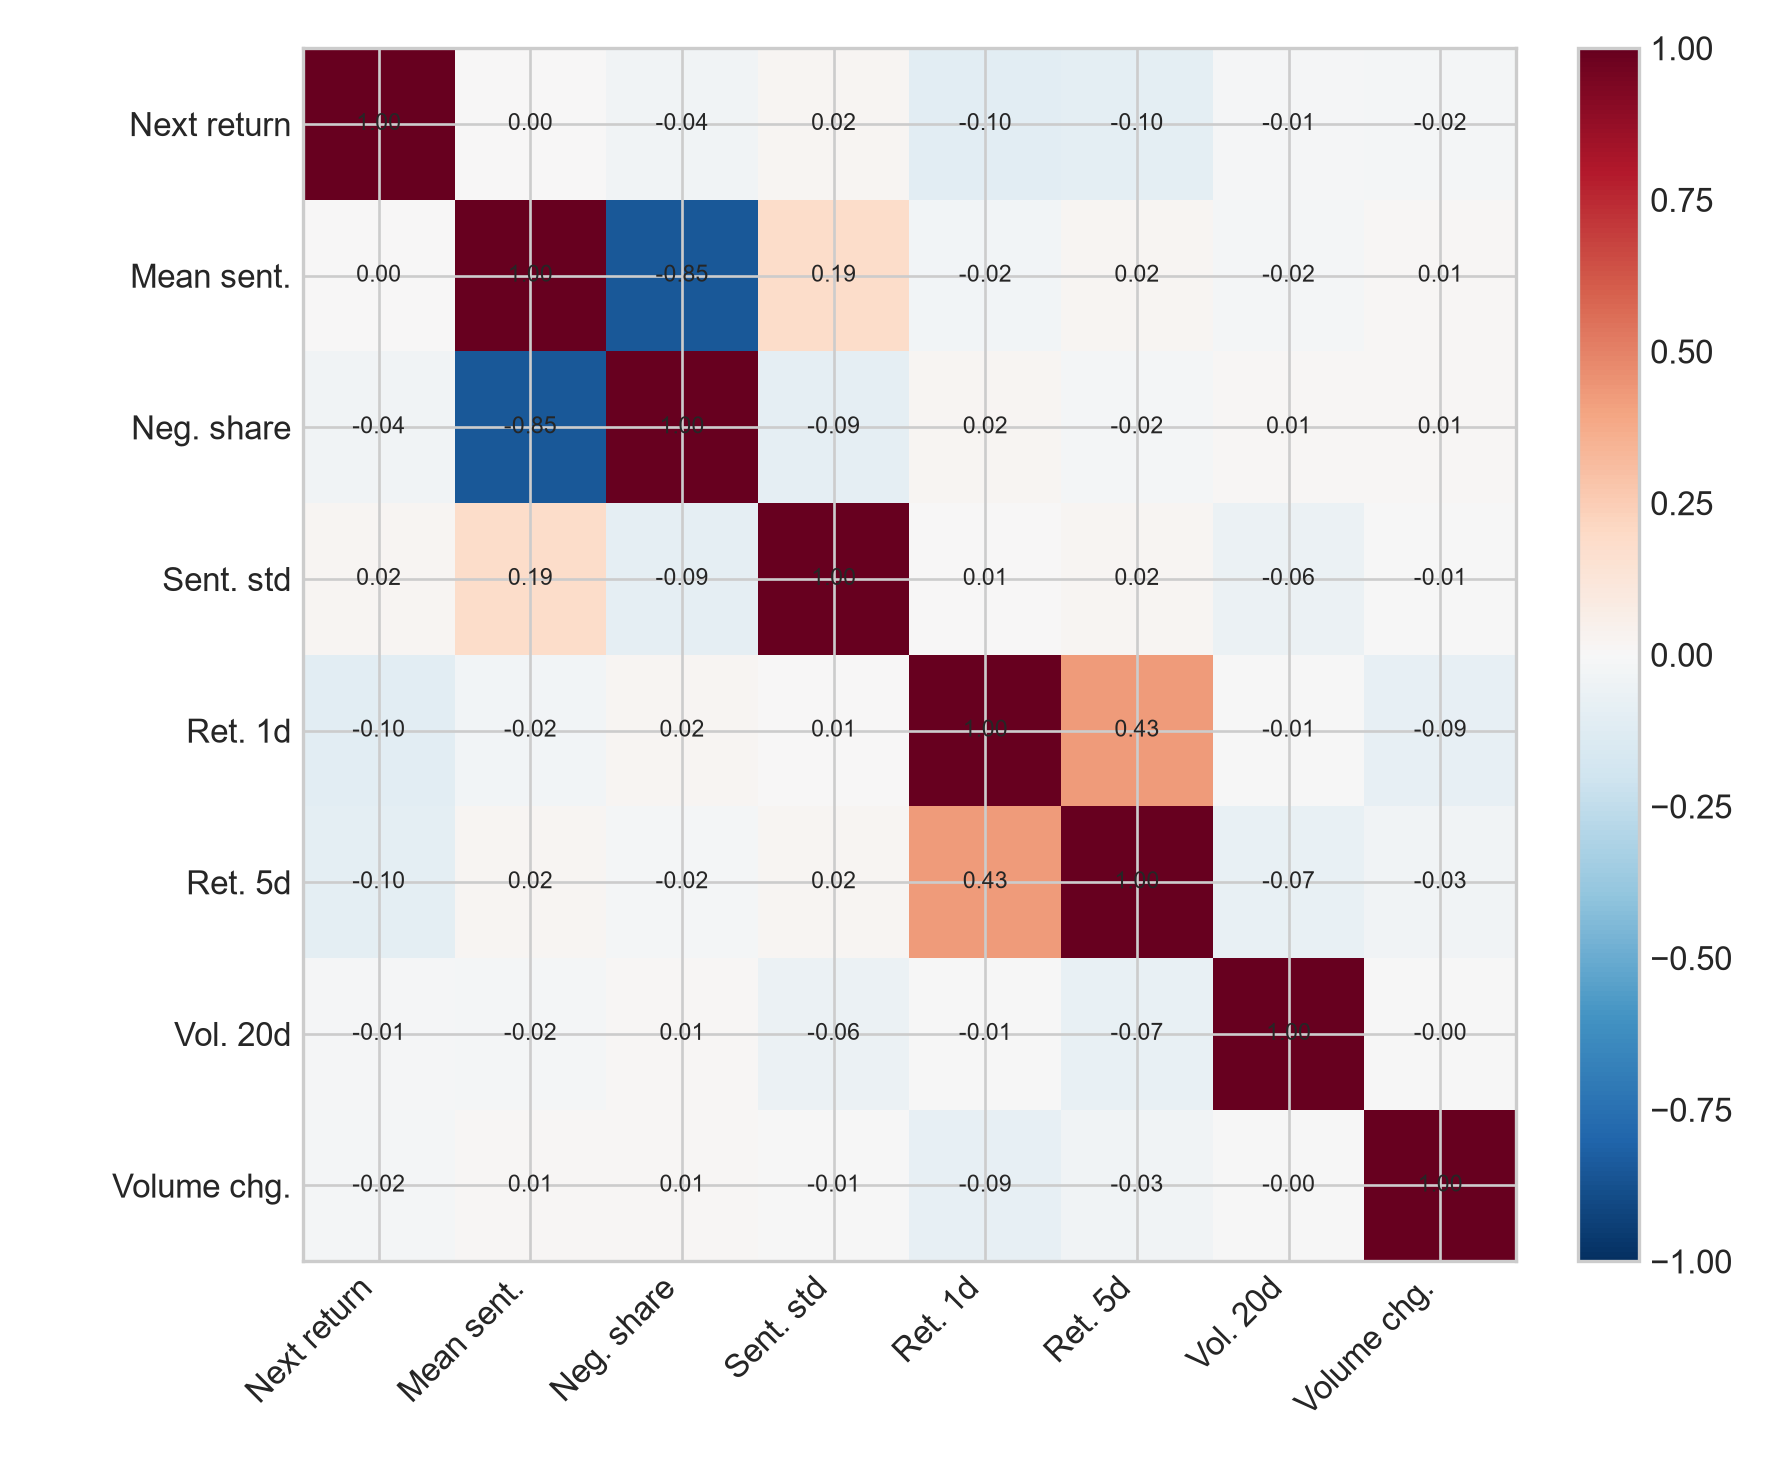
\includegraphics[width=\columnwidth]{figures/feature_correlation.png}
\caption{主要新闻、量价变量与下一日收益的相关系数}
\label{fig:corr}
\end{figure}

\section{研究方法}

\subsection{模型与特征消融}

Logistic回归作为线性基准并设置类别权重；随机森林使用500棵树、最大深度5和
最小叶节点12；XGBoost使用350棵深度3的树、学习率0.025、0.8行列采样以及
$L_1/L_2$正则化\cite{xgboost}。设置：
\begin{itemize}
  \item P：仅量价和技术指标；
  \item P+N：P加新闻情绪、占比、分歧和滞后变量。
\end{itemize}
同一算法的P+N与P之差用于检验H1。

\subsection{时间序列验证}

测试年份为2014、2015和2016。每折用测试年前一年验证、更早样本训练，并在验证与
测试开始前设置20个交易日隔离期。例如2015折使用2013年及以前训练、2014年验证、
2015年测试。所有填补、标准化和模型拟合只使用训练数据。分类阈值在验证集上最大化
F1，再固定到测试集。

这种walk-forward设计更接近真实部署。随机交叉验证会把未来市场状态混入训练，
重叠滚动窗口还可能产生额外泄漏\cite{lop}。

\subsection{指标与显著性}

主要指标为ROC-AUC和平衡准确率，辅助指标为PR-AUC、F1与Brier分数。F1容易因模型
大量预测上涨而偏高，因此不能单独解释。对XGBoost两组的同日预测进行2000次配对
bootstrap，获得AUC增量的95\%置信区间。

\subsection{经济性检验}

当P+N模型预测上涨概率$p_t\geq0.55$时持有DJIA，否则持有现金：
\begin{equation}
R_{t+1}^{net}=I(p_t\geq0.55)r_{t+1}-0.001|\Delta w_t|.
\end{equation}
其中$w_t$为仓位，0.001代表每次仓位变化10个基点成本。报告年化收益、年化波动、
夏普比率、最大回撤和持仓比例。

\section{实验结果}

\subsection{平均样本外表现}

\begin{table}[t]
\centering
\caption{2014--2016年测试窗口平均结果}
\scriptsize
\setlength{\tabcolsep}{2.5pt}
\begin{tabular}{llccccc}
\toprule
模型 & 特征 & AUC & PR-AUC & F1 & BAcc & Brier\\
\midrule
LR & P & .493 & .533 & .699 & .500 & .251\\
LR & P+N & .489 & .551 & .692 & .498 & .252\\
RF & P & .471 & .561 & .699 & .503 & .253\\
RF & P+N & .485 & .540 & .694 & .494 & .251\\
XGB & P & .472 & .551 & .680 & .489 & .263\\
XGB & P+N & \textbf{.504} & .555 & .695 & .501 & .256\\
\bottomrule
\end{tabular}
\label{tab:result}
\end{table}

表\ref{tab:result}显示，所有AUC接近0.5。Logistic加入新闻后下降0.004，随机森林
提高0.014，XGBoost提高0.032。新闻可能通过非线性交互提供有限信息，但整体方向
识别能力仍接近随机。

\begin{figure*}[t]
\centering
\begin{subfigure}[t]{0.48\textwidth}
  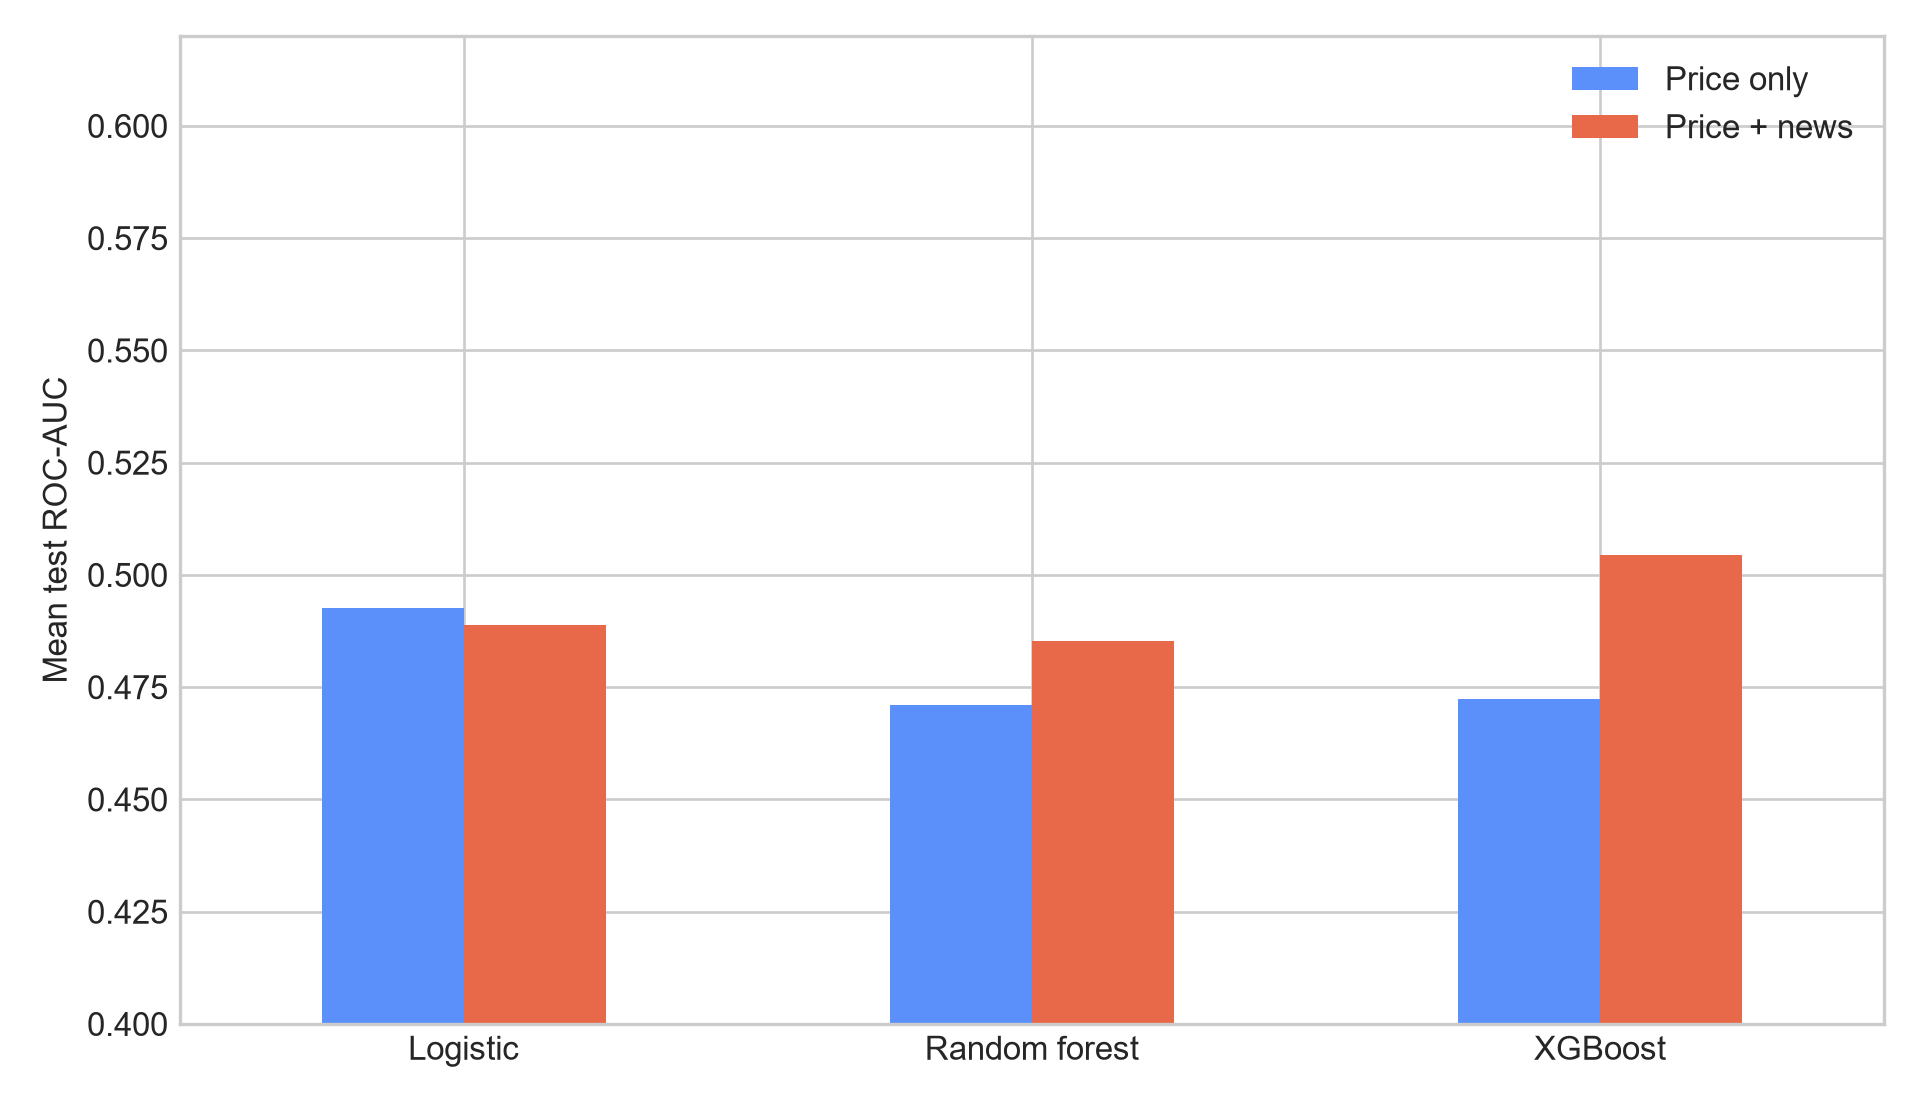
\includegraphics[width=\linewidth]{figures/model_auc_comparison.png}
  \caption{三类模型的平均AUC}
\end{subfigure}
\hfill
\begin{subfigure}[t]{0.48\textwidth}
  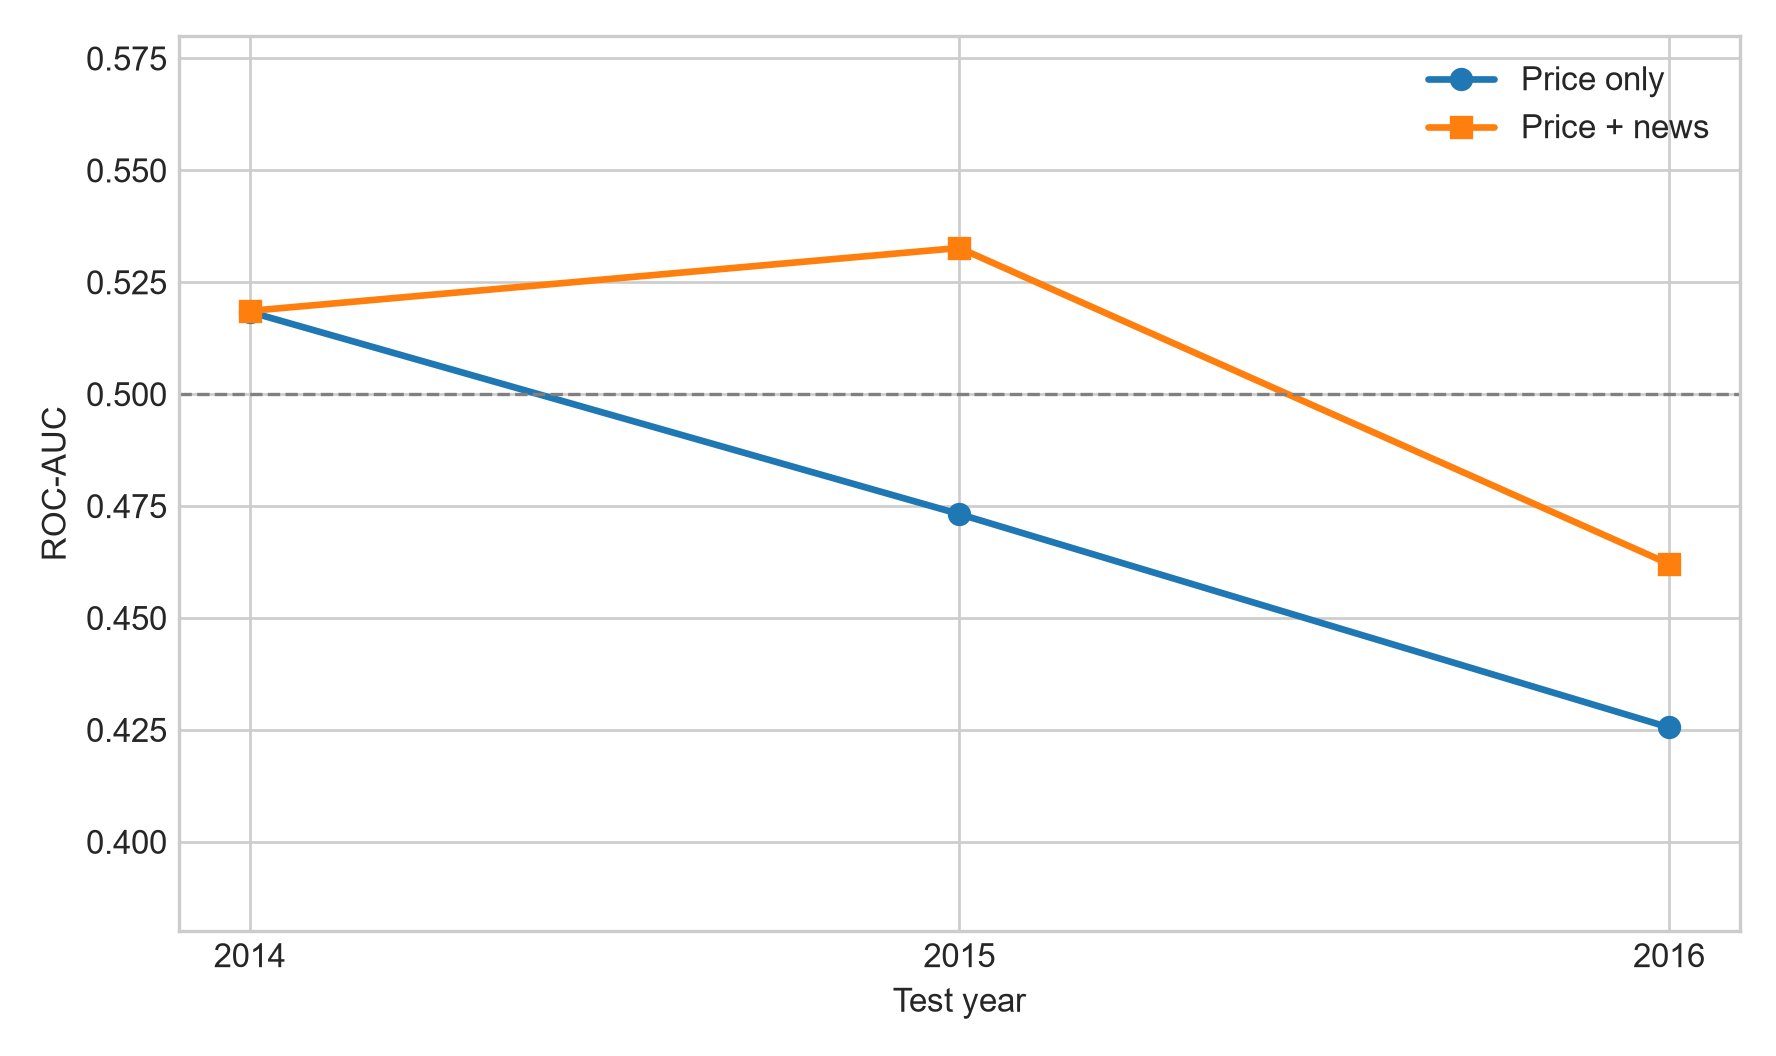
\includegraphics[width=\linewidth]{figures/yearly_xgboost_auc.png}
  \caption{XGBoost逐年AUC}
\end{subfigure}
\caption{加入新闻前后的平均表现与年度稳定性}
\label{fig:auc}
\end{figure*}

\subsection{年度稳定性与显著性}

XGBoost P+N在2014、2015和2016年的AUC分别为0.519、0.533和0.462；P模型分别为
0.518、0.473和0.426。新闻在2015年改善较明显，但2016年两组均低于0.5，H2不成立。
将575个样本外预测合并，AUC增量为0.0348，95\%置信区间为
$[-0.0060,0.0734]$，包含0，故H1仅获得方向性证据，未获得统计显著支持。

\begin{figure}[t]
\centering
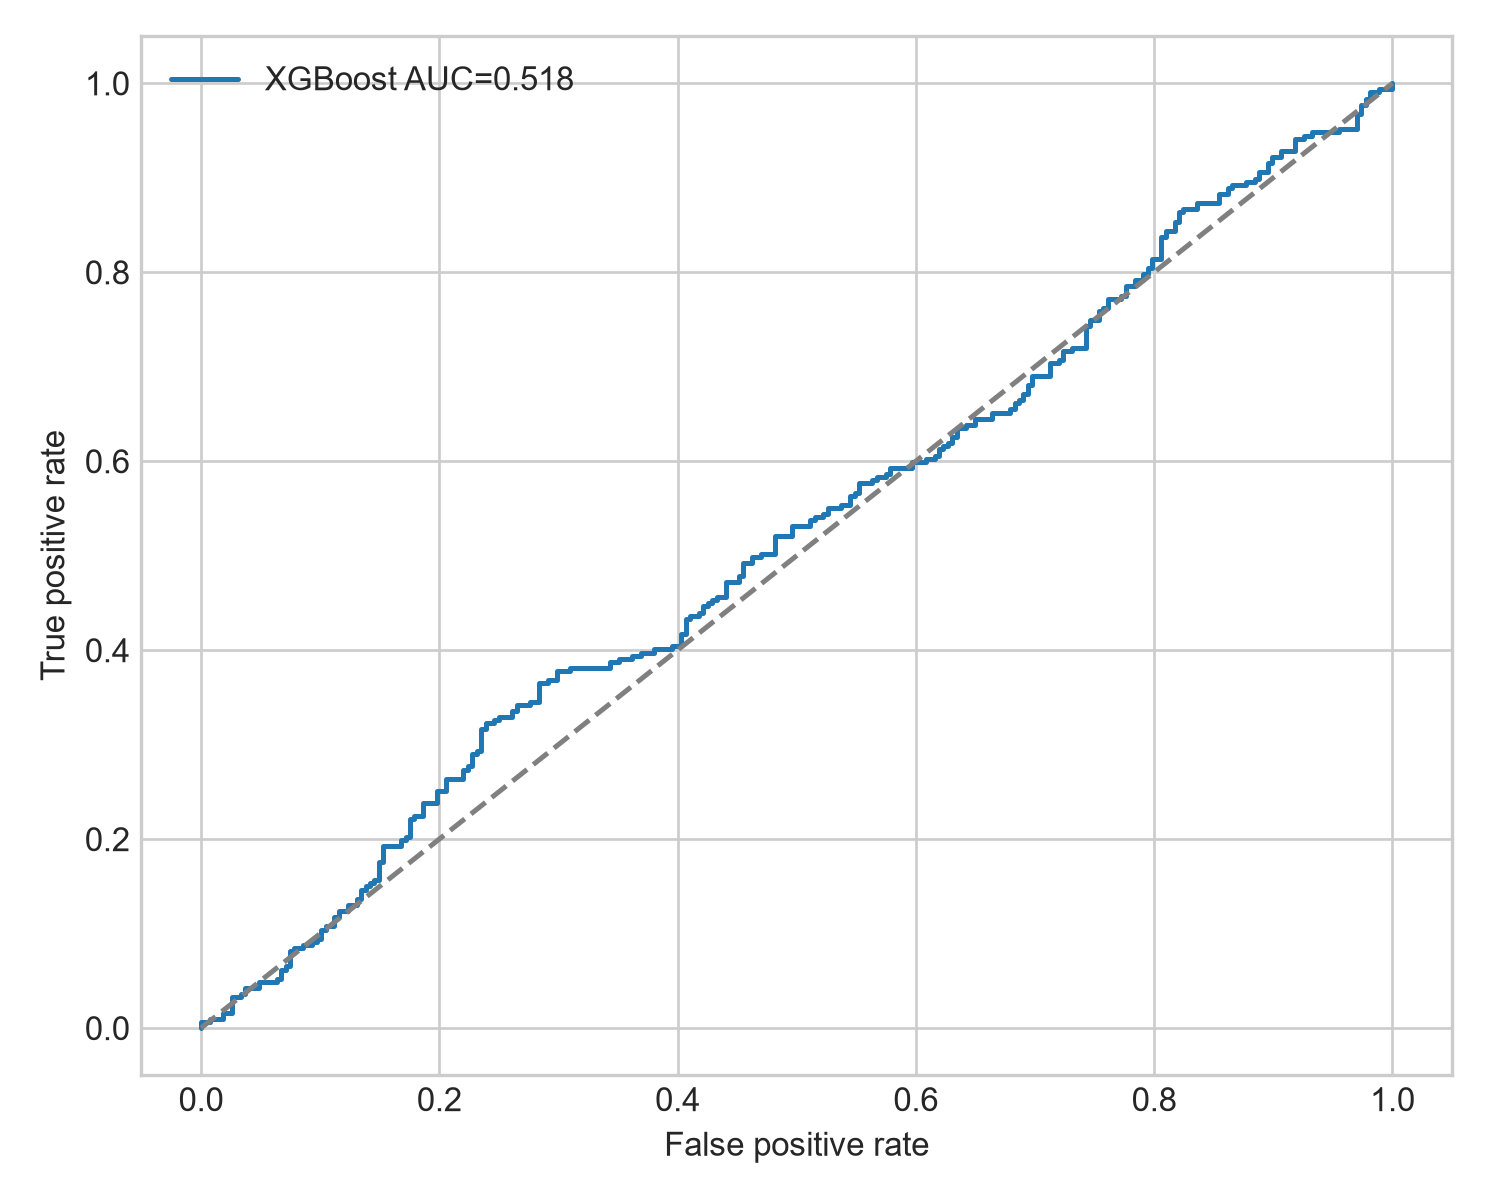
\includegraphics[width=0.90\columnwidth]{figures/xgboost_roc_curve.png}
\caption{XGBoost P+N模型合并测试期ROC曲线}
\label{fig:roc}
\end{figure}

合并测试期ROC-AUC为0.518，高于逐年AUC简单平均0.504，是因为不同年份样本数和
预测分布不同。两者均说明辨别能力较弱，不能将0.5附近的数值解释为稳定优势。

\subsection{概率校准与阈值敏感性}

分类排序能力并不等于概率可靠。图\ref{fig:calibration}显示各概率分箱的实际上涨
频率围绕理想线明显波动，Brier分数为0.256，略差于无信息概率基准附近水平。
这意味着0.60的预测概率并不稳定对应60\%上涨频率。

\begin{figure*}[t]
\centering
\begin{subfigure}[t]{0.48\textwidth}
  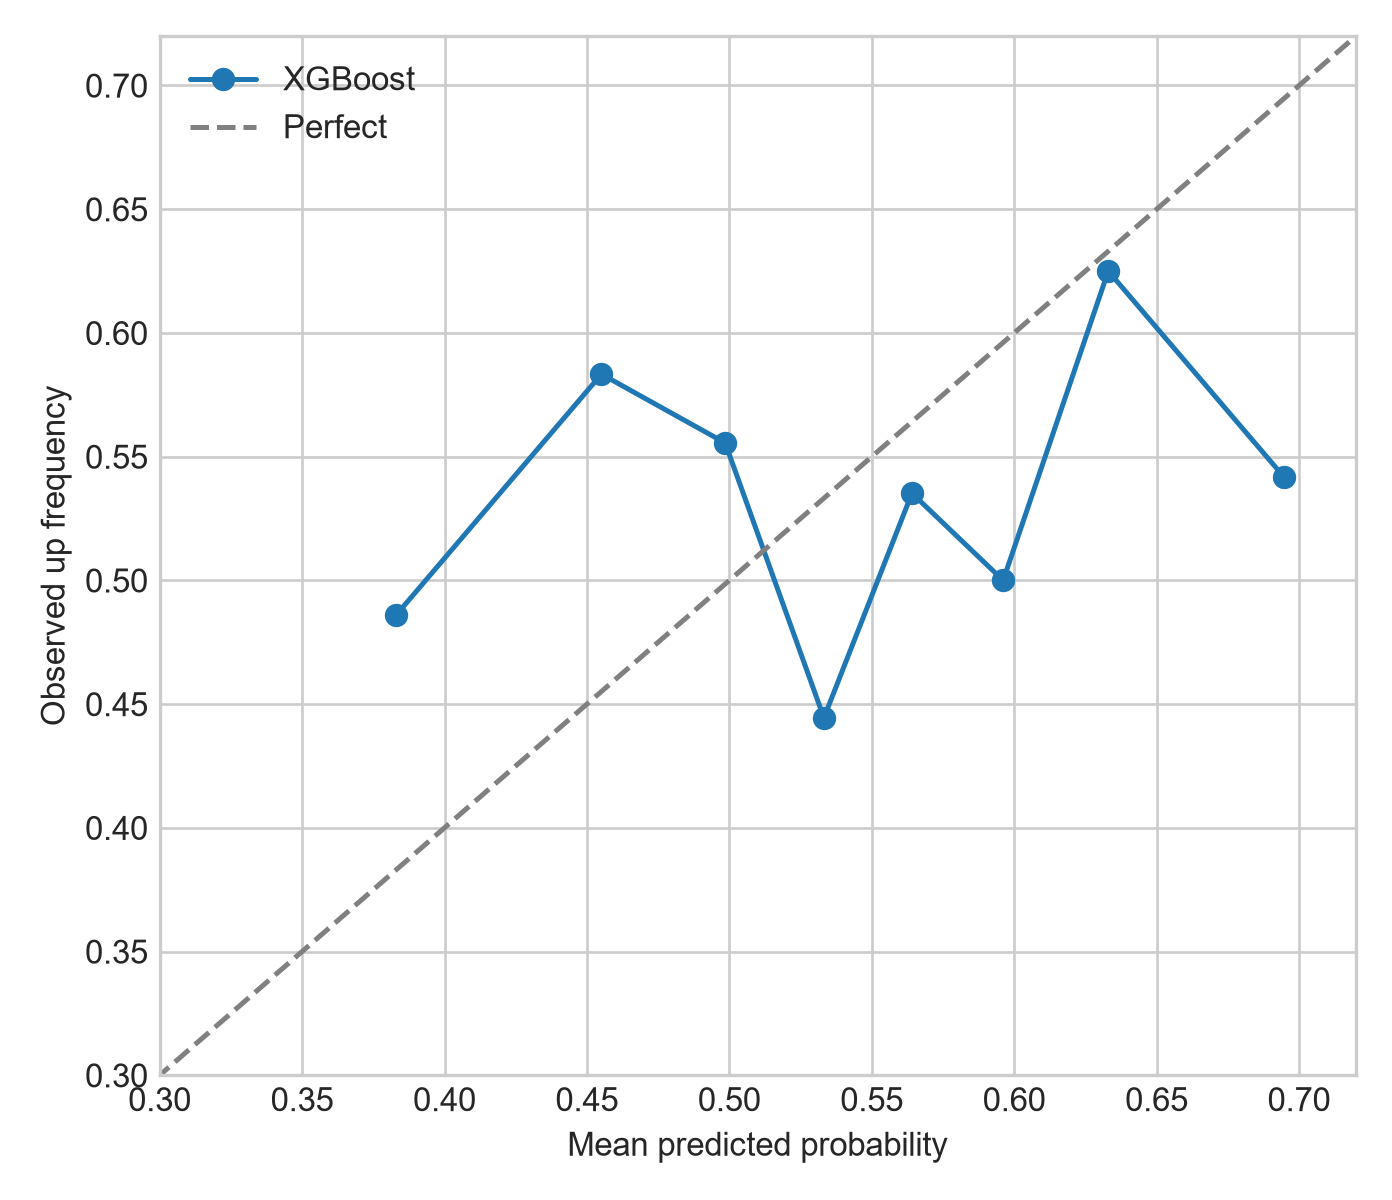
\includegraphics[width=\linewidth]{figures/calibration_curve.png}
  \caption{概率校准曲线}
\end{subfigure}
\hfill
\begin{subfigure}[t]{0.48\textwidth}
  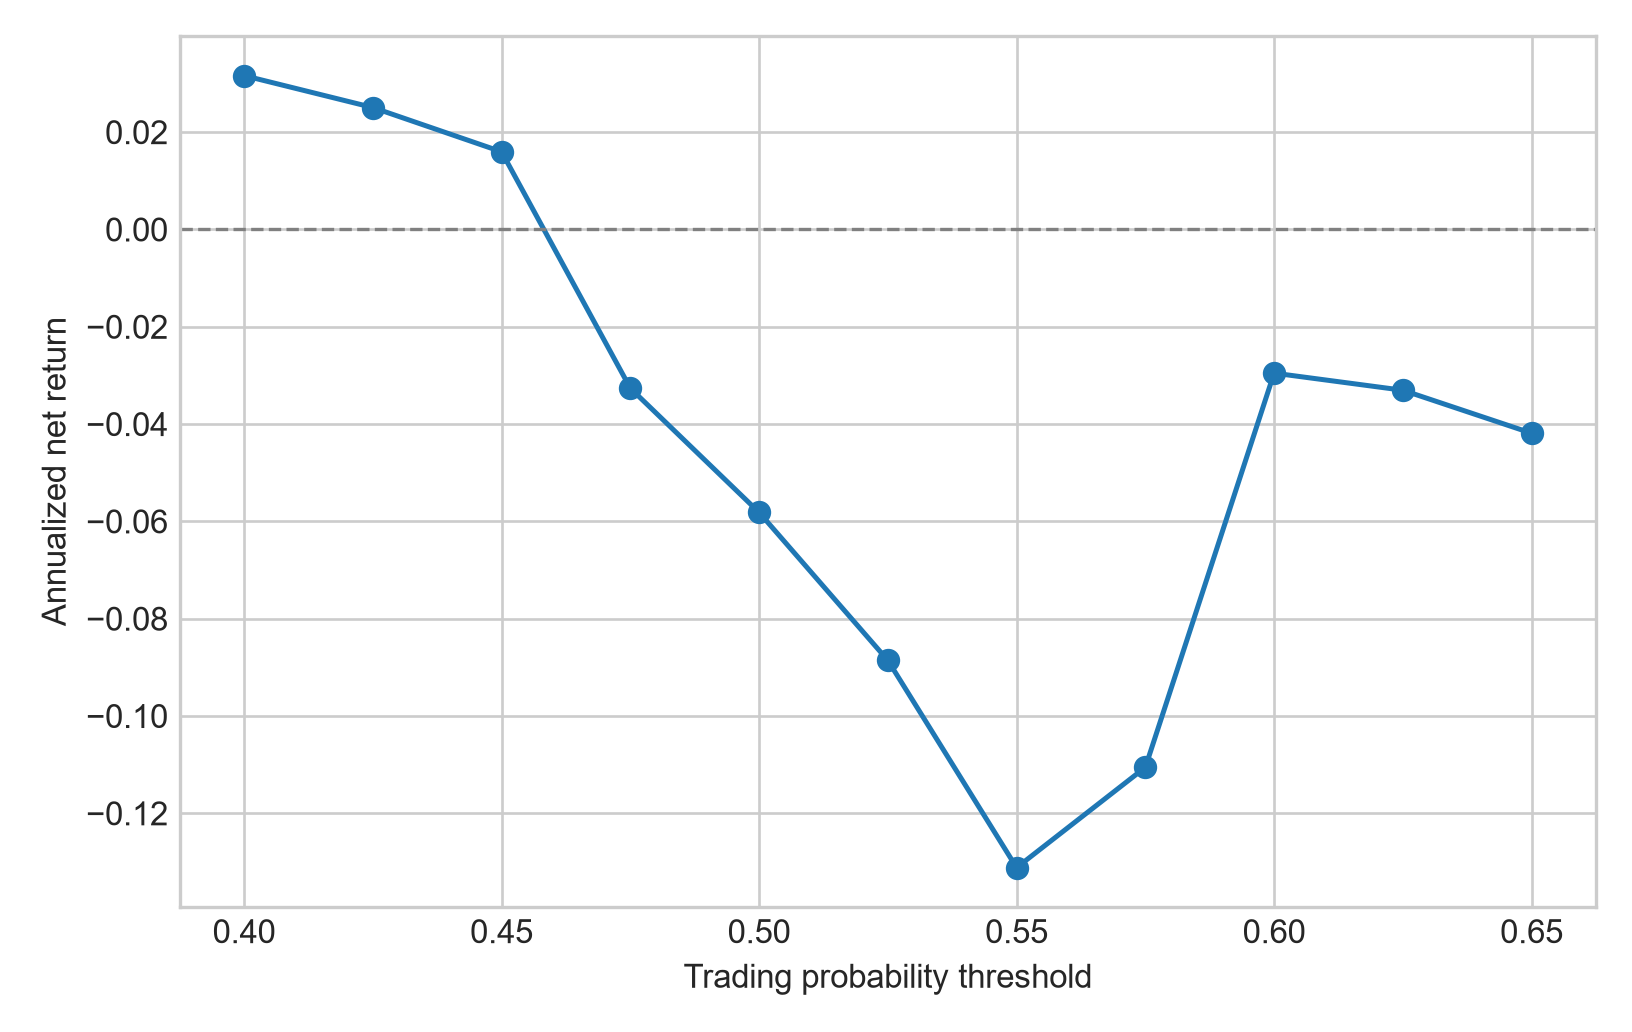
\includegraphics[width=\linewidth]{figures/threshold_sensitivity.png}
  \caption{交易阈值与年化净收益}
\end{subfigure}
\caption{XGBoost P+N模型的概率质量和阈值敏感性}
\label{fig:calibration}
\end{figure*}

阈值从0.40提高到0.65时，年化净收益大幅变化。0.40--0.45附近出现小幅正收益，
但该范围意味着高持仓比例，且阈值0.475之后大多为负。结果对人为阈值高度敏感，
无法支持稳定策略。

\subsection{经济性结果}

\begin{table}[t]
\centering
\caption{XGBoost新闻策略经济指标}
\small
\begin{tabular}{lr}
\toprule
指标 & 数值\\
\midrule
样本外交易日 & 575\\
持仓比例 & 48.52\%\\
年化净收益 & $-13.12\%$\\
年化波动率 & 8.69\%\\
夏普比率 & $-1.51$\\
最大回撤 & $-29.46\%$\\
DJIA买入持有年化收益 & 8.95\%\\
\bottomrule
\end{tabular}
\label{tab:strategy}
\end{table}

图\ref{fig:return}显示新闻策略从2014年起持续落后，2015年市场波动期间回撤明显。
统计上的微弱排序提升没有转化为经济收益，H3不成立。

\begin{figure*}[t]
\centering
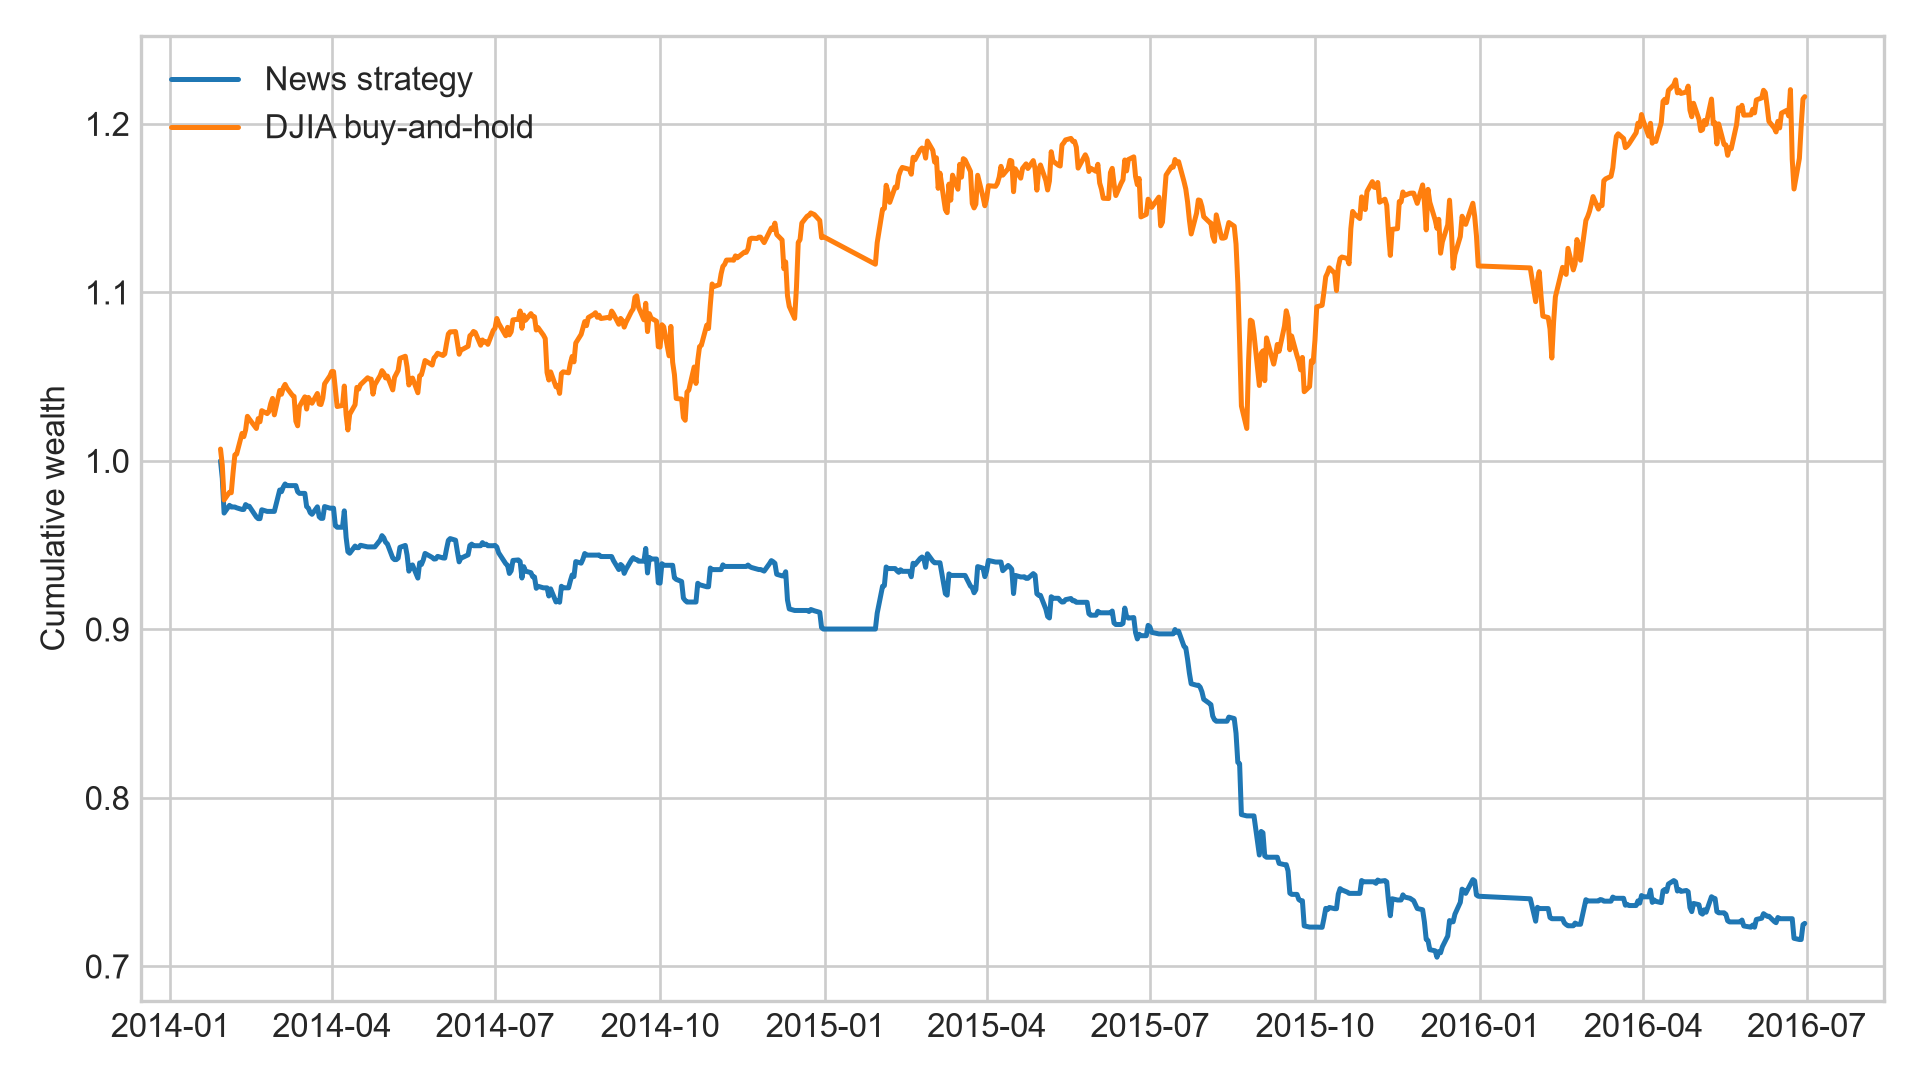
\includegraphics[width=0.80\textwidth]{figures/cumulative_returns.png}
\caption{新闻策略与DJIA买入持有的样本外累计净值}
\label{fig:return}
\end{figure*}

\section{讨论}

\subsection{为什么新闻信号较弱}

第一，标题是Reddit筛选的全球热点，包含战争、政治和社会事件，不完全对应DJIA
成分公司。公司级新闻与个股价格的映射比“全球新闻--指数”映射更直接。第二，
VADER未在金融语料训练，对盈利预警、评级变化和并购条款的理解弱于FinBERT。
第三，日均聚合会抵消同日正负事件，且丢失新闻排序、主体和事件类型。第四，公开
新闻可能快速入价，日频下一日预测窗口过长。第五，市场机制随年份变化，导致
2014--2015的弱信号无法延续至2016。

\subsection{与既有研究的关系}

本文结果并不否定新闻文本的研究价值，而是界定了低粒度数据和简单情绪聚合的边界。
Ding等的事件表示保留主体与动作\cite{ding2015}，StockNet保留文本序列和价格动态
\cite{stocknet}，FinBERT提供金融领域语义\cite{finbert}，FNSPID与CausalStock
提供公司级大样本和关系信息\cite{fnspid,causalstock}。相比之下，本研究更接近
一个严格验证的教学基线。其价值在于说明：若没有精确时间戳、公司映射和更丰富文本
表示，增加复杂分类器并不能自动获得可交易信号。

\section{稳健性、局限与扩展}

本文已完成三类稳健性诊断：逐年AUC比较、bootstrap置信区间、不同交易阈值回测。
结果均指向信号不稳定。仍有以下局限：
\begin{enumerate}
  \item 新闻缺少精确发布时间，无法区分盘前、盘中和盘后；
  \item 样本仅约2000日，2016测试期只有上半年；
  \item VADER不是金融领域模型，且未利用完整文本；
  \item 回测使用DJIA指数收益，未包含滑点与实际产品跟踪误差；
  \item 固定超参数减少了数据窥探，但可能不是每折最优参数。
\end{enumerate}

后续研究应优先改进数据而非盲目堆叠模型：使用FNSPID等带时间戳和股票代码的数据；
以FinBERT或Financial PhraseBank微调模型提取情绪；保留新闻来源、排名、主体和
事件类别；分别预测盘前到收盘、收盘到次日开盘等窗口；使用历史指数成分和行业关系；
以超过交易成本的收益阈值构造标签；采用概率校准及purged/embargo验证。

\section{结论}

本文以1968个交易日和49193条标题构建了新闻情绪与DJIA量价融合的下一日方向预测。
严格walk-forward结果显示，XGBoost加入新闻后平均AUC由0.472提高至0.504，但
bootstrap置信区间包含0；逐年表现不稳定，概率校准较差，0.55阈值策略年化收益
$-13.1\%$。因此，该数据和VADER聚合方法至多提供微弱、时变的非线性信息，不足以
支持稳定预测或交易应用。研究说明，金融机器学习中时间对齐、样本外验证和经济检验
比单纯提高模型复杂度更重要。

\begin{thebibliography}{99}\scriptsize
\bibitem{tetlock}
Tetlock, P. C. Giving Content to Investor Sentiment: The Role of Media in the Stock Market.
\emph{The Journal of Finance}, 62(3):1139--1168, 2007.

\bibitem{lm}
Loughran, T., McDonald, B. When Is a Liability Not a Liability? Textual Analysis,
Dictionaries, and 10-Ks. \emph{The Journal of Finance}, 66(1):35--65, 2011.

\bibitem{phrasebank}
Malo, P., Sinha, A., Korhonen, P., Wallenius, J., Takala, P.
Good Debt or Bad Debt: Detecting Semantic Orientations in Economic Texts.
\emph{JASIST}, 65(4):782--796, 2014.

\bibitem{vader}
Hutto, C. J., Gilbert, E. VADER: A Parsimonious Rule-based Model for Sentiment
Analysis of Social Media Text. \emph{ICWSM}, 2014.

\bibitem{ding2015}
Ding, X., Zhang, Y., Liu, T., Duan, J. Deep Learning for Event-Driven Stock Prediction.
\emph{IJCAI}, 2015.

\bibitem{stocknet}
Xu, Y., Cohen, S. B. Stock Movement Prediction from Tweets and Historical Prices.
\emph{ACL}, 2018.

\bibitem{akita}
Akita, R., Yoshihara, A., Matsubara, T., Uehara, K.
Deep Learning for Stock Prediction Using Numerical and Textual Information.
\emph{IEEE/ACIS ICIS}, 2016.

\bibitem{finbert}
Araci, D. FinBERT: Financial Sentiment Analysis with Pre-trained Language Models.
arXiv:1908.10063, 2019.

\bibitem{fnspid}
Dong, Z., Fan, X., Peng, Z. FNSPID: A Comprehensive Financial News Dataset in Time Series.
arXiv:2402.06698, 2024.

\bibitem{causalstock}
Soun, Y., et al. CausalStock: Deep End-to-end Causal Discovery for News-driven
Stock Movement Prediction. \emph{NeurIPS}, 2024.

\bibitem{rf}
Breiman, L. Random Forests. \emph{Machine Learning}, 45:5--32, 2001.

\bibitem{xgboost}
Chen, T., Guestrin, C. XGBoost: A Scalable Tree Boosting System.
\emph{KDD}, 785--794, 2016.

\bibitem{lop}
L\'opez de Prado, M. \emph{Advances in Financial Machine Learning}. Wiley, 2018.

\bibitem{dataset}
Sun, J. Daily News for Stock Market Prediction, Version 1. Kaggle, 2016.
\url{https://www.kaggle.com/datasets/aaron7sun/stocknews}.
\end{thebibliography}

\end{document}
